\section{Nucleation crowding and diversity}
\label{S-sec:s-crowding}

We measure candidate crowding, correct-pose coverage among the first $k$ candidates (\cref{S-fig:s-crowding}b), and the cost and sensitivity of site capacity. Unless stated otherwise, the results use the training cohort of 3000 FPFH pairs from 82 3DMatch training scenes.

\begin{table*}[t]
\caption{Same-budget diversity controls on 3000 training pairs. Distinct and Cov.@1024 measure raw candidates; Ceiling measures the refined pool and Reg. the released result. Time is relative to NGRR-LS in this run.}
\label{S-tab:s-diversity}

\centering\small
\begin{tabular}{lrrrrr}
\toprule
Second half & Distinct $\uparrow$ & Cov.@1024 $\uparrow$ & Ceiling $\uparrow$ & Reg. $\uparrow$ & Time \\
\midrule
ranking (\ngr{}) & 222.6 & 2528 & 2429 & 2298 & -- \\
site capacity (\ls{}) & \textbf{409.6} & \textbf{2639} & \textbf{2487} & \textbf{2326} & 1.00 \\
MMR, $\lambda=\frac12$ & 337.8 & 2624 & \textbf{2487} & \textbf{2326} & 0.94 \\
hard capacity & 363.2 & 2615 & 2467 & 2312 & 0.90 \\
pose NMS & 243.0 & 2547 & 2438 & 2310 & 0.91 \\
\bottomrule
\end{tabular}

\end{table*}

\paragraph{The crowding statistic.} We diagnose crowding stage by stage on the training cohort. Ground truth is used to label candidates only after the frontend has run. True inliers are the matches whose residual under the ground-truth pose is below $\tau=0.1$\,m, and a triple is pure if all three of its matches are true inliers. For each pair, the stages of the original \ngr{} frontend are rerun unchanged. Among the 372 pairs with at most 25 true inliers, the 1024 kept nuclei contain a pure triple for 95 pairs, whereas a deeper ranking of 16\,384 triples contains one for 189. This ranking uses the same affinity $T_{abc}$ and the same per-block search over shortlisted pairs. The difference is consistent with crowding (\main{\cref*{sec:capacity}}), although this statistic alone does not establish the mechanism.

\begin{figure*}[t]
\centering
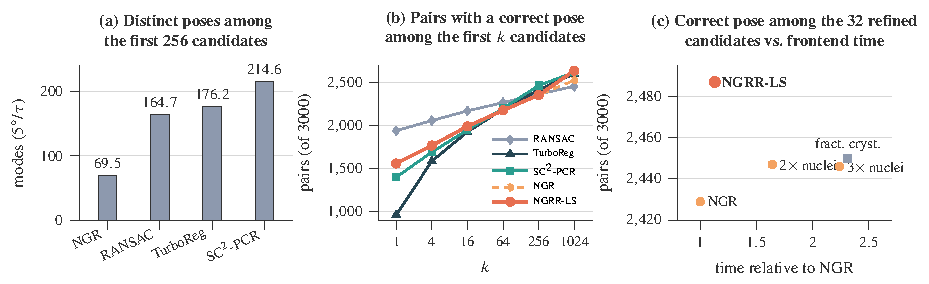
\includegraphics[width=.92\linewidth]{shared/figures/fig_crowding.pdf}
\caption[Nucleation crowding on the training cohort]{Nucleation crowding on the 3DMatch training cohort (3000 pairs, FPFH). (a) \ngr{}'s first 256 candidates contain few distinct poses; \ls{} keeps the same first half by construction. (b) Pairs with a correct pose among the first $k$ candidates before finishing: \ls{} departs from \ngr{} only beyond rank 256 and overtakes every baseline at 1024. (c) Pairs with a correct pose among up to 32 refined candidates against frontend run time, relative to \ngr{}: doubling or tripling the nuclei or fractional crystallization adds 17--21 pairs at 1.6--2.3$\times$ the time; the finite site capacity adds 58 at 1.13$\times$. Panels (a) and (c) are summarized in \main{\cref*{sec:crowding}}.}
\label{S-fig:s-crowding}
\end{figure*}

\paragraph{Crowding on the ranked candidates.} \ngr{}'s first 256 candidates contain only 69.5 distinct poses (greedy, at $5^\circ$ and $\tau$), a third of SC$^2$-PCR's 214.6; RANSAC has 164.7 and TurboReg 176.2. From rank 64 on, SC$^2$-PCR and TurboReg cover more pairs with a correct pose (\cref{S-fig:s-crowding}b; a candidate counts if it lies within $15^\circ$ and 0.3\,m of the ground truth, before finishing). Doubling or tripling the nucleus budget retains the original ranking and adds 18 and 17 pairs with a correct refined candidate, at 1.64$\times$ and 2.24$\times$ the frontend time. Fractional crystallization (harvesting the main crystal and renucleating from the depleted liquor) adds 21 at 2.31$\times$ the time. The finite site capacity raises coverage at rank 1024 from 2528 to 2639 pairs and the refined-pool ceiling from 2429 to 2487 ($+71/-13$, $p=8\times10^{-11}$), at 1.13$\times$ the run time. It was the only one of the four pre-registered candidate variants to pass the adoption rule; the doubled and tripled budgets were pre-registered as controls.

\paragraph{Test cohorts.} On the nine frozen test cohorts the ceiling rises from 10\,158 to 10\,292 pairs. The release assay converts this coverage gain into 9857 $\to$ 9920 registered pairs ($+121/-58$ paired, $p=3\times10^{-6}$). With the learned assay, the counts are 9969 $\to$ 10\,084 ($+199/-84$, $p=6\times10^{-12}$). The finishing step's anchor rule yields a smaller gain (9724 $\to$ 9752, $p=0.037$).

\paragraph{Site capacity against other diversity rules.} The controls in \cref{S-tab:s-diversity} keep \ls{}'s budget, first halves and deep rankings (65\,536 pairs, 16\,384 triples) and the same $K$, and fill the second halves using three alternative selection rules (defined in \cref{S-sec:s-method}). This comparison was added after the main evaluation; each rule was pre-registered before it was run, and the comparison does not change the reported pipeline. The columns of the table are: Distinct, the mean number of distinct poses ($5^\circ$, $\tau$) among the first 1024 candidates; Cov.@1024, pairs with a strictly correct pose among them; Ceiling, pairs with a correct pose among up to 32 refined candidates; Reg., pairs registered after finishing and the release assay; and Time, the mean frontend time relative to \ls{} in the same run. MMR is maximal marginal relevance on the match sets. The \ls{} row matches the pre-registered run (ceiling 2487).

Maximal marginal relevance, with its default trade-off $\lambda=\frac12$, reaches exactly the same ceiling as the site capacity (2487 pairs, $+16/-16$) and the same final count (2326, $+13/-13$), with fewer distinct poses (338 against 410 among the first 1024). A hard capacity (a match may sit in at most 8 pairs or 4 triples) runs out of admissible motifs in 1187 of the 3000 pairs and fills the remaining slots in ranking order. Its coverage is lower by 20 pairs ($+9/-29$, Holm $p=0.008$). Suppressing nuclei whose three-point pose repeats an earlier one loses 49 ($+10/-59$, Holm $p=8\times10^{-9}$) and only slightly increases the number of distinct poses (243, against 223 for \ngr{}): nuclei with different seed poses still grow into the same few modes. After verification the differences shrink (2312 and 2310 registered pairs against 2326; Holm $p=0.05$ and $0.08$). These controls support soft penalties on shared matches as a way to reduce crowding.

\paragraph{Cost and constants.} On the training cohort the site capacity adds 13\% to the frozen frontend time (mean time ratio 1.13), doubling the nuclei 64\%. These are mean ratios relative to \ngr{}, as in \cref{S-fig:s-crowding}c; the Time column of \cref{S-tab:s-diversity} is relative to \ls{} in the same run, and the median times in \main{\cref*{tab:joint}} come from 100 3DLoMatch+FPFH pairs. Halving or doubling either site-capacity constant changes the refined-pool ceiling and the final count on 1000 training pairs by at most three pairs. The capacities $q=8$ for pairs and $q=4$ for triples were fixed when the variant was pre-registered and never tuned.
